\chapter{Softwarearchitektur}

\section{Clean Architecture}

Die Applikation orientiert sich an einer geschichteten Architektur, die Elemente der Clean Architecture aufgreift:

\begin{itemize}
    \item \textbf{Domain / Entities (innerster Ring):}
    Die Memory-Abstraktion (\code{Bit}, \code{Nibble}, \code{Byte}, \code{Register}) sowie \code{Ram}, \code{Stack} und \code{MemoryInterface}.
    Diese Klassen modellieren die Hardwaredomäne des PIC-Mikrocontrollers und haben keine Abhängigkeiten zu Framework- oder UI-Code.
    \item \textbf{Use Cases / Application Layer:} \code{Instruction} (mit allen 35+ Unterklassen), \code{ALU}, \code{Compiler},
    \code{Program}, \code{Timer}, \code{Prescaler} und \code{PIC}. Diese Schicht orchestriert die Simulation und nutzt die Domain-Klassen.
    \item \textbf{Interface Adapters:} \code{Filereader} (Dateisystem-Zugriff), \code{Logger} (Ausgabe-Abstraktion).
    \item \textbf{Frameworks / UI (äußerster Ring):} \code{TerminalUI}, \code{TUI_Renderer},
    \code{TUI_Controller} und alle TUI-Hilfsklassen. Diese hängen von ncurses ab und nutzen \code{PICSnapshot} als Daten-Transfer-Objekt.
\end{itemize}

\begin{center}
    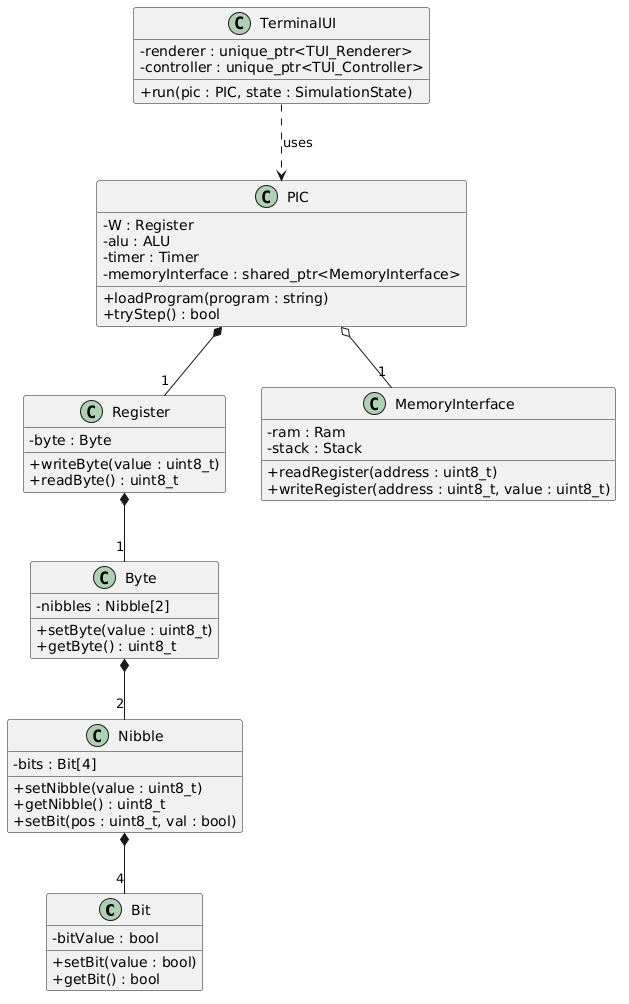
\includegraphics[width=0.9\textwidth]{UML/1.png}
\end{center}

\section{Domain Code}

\textbf{Domain Code} ist Code, der die überall gültige Logik der Anwendungsdomäne abbildet, unabhängig von Frameworks, Datenbanken oder UI.
Er ist der innere Teil der Anwedung, der sich selten ändern sollte. Im Fall von PICasso ist die Domäne die PIC-Mikrocontroller-Hardware.

\textbf{Beispiel:} Die Klasse \code{Stack} (\code{header/stack.hpp}) modelliert den 8-Level-Hardware-Stack des PIC. Sie hat keine Abhängigkeiten zu externen Bibliotheken und bildet rein fachliche Hardware-Logik ab:

\begin{lstlisting}[style=codeblock,language=picassocpp]
class Stack {
    private:
        uint8_t stack[8];
        uint8_t stackPointer;
    public:
        Stack();
        void push(uint8_t value);
        uint8_t pop();
        void reset();
};
\end{lstlisting}

\section{Analyse der Dependency Rule}
\subsection{Positiv-Beispiel: Dependency Rule}

Die Klasse \code{Register} (Domain/Entity) hat keine Abhängigkeiten zu äußeren Schichten.
Sie hängt nur von \code{Byte} ab, welches wiederum nur von \code{Nibble} und \code{Bit} abhängt welche alle innerhalb der Domain-Schicht sind.
Die äußere Schicht \code{Ram} hängt von \code{Register} ab, aber \code{Register} weiß nichts von \code{Ram}.
Die Abhängigkeit zeigt korrekt von außen nach innen.

\begin{center}
    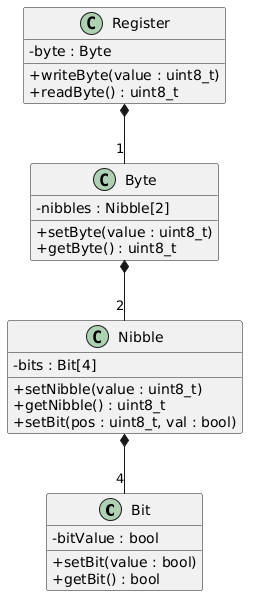
\includegraphics[width=0.5\textwidth]{UML/2.png}
\end{center}

\subsection{Negativ-Beispiel: Dependency Rule}

Die abstrakte Klasse \code{Instruction} (Application Layer) hat ein \textbf{statisches} Feld \code{static std::shared_ptr<MemoryInterface> memoryInterface},
das durch die \code{PIC}-Klasse gesetzt wird.
Das bedeutet, dass die Application-Layer-Klasse \code{Instruction} direkt an die konkrete Implementierung \code{MemoryInterface} gekoppelt ist.
Zudem wird das statische Feld von \code{PIC} (einem Orchestrator) gesetzt was zu einer impliziten Abhängigkeit von außen nach innen, 
die zur Laufzeit besteht, obwohl die Instruction-Klasse eigentlich keine Kenntnis über PIC haben sollte, führt.

\textbf{Lösung:} Dependency Injection -- die \code{MemoryInterface}-Referenz sollte als Konstruktor-Parameter an jede Instruction übergeben werden, statt über ein statisches Feld.

\begin{center}
    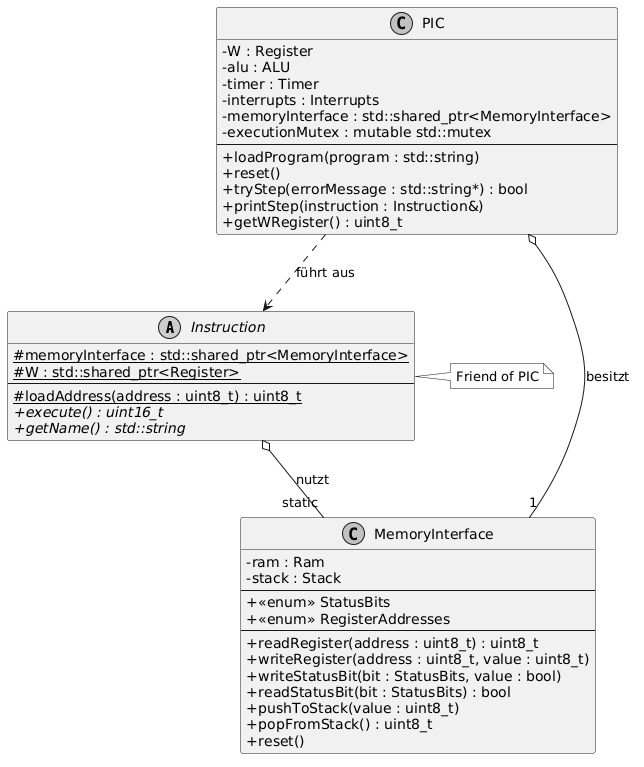
\includegraphics[width=0.9\textwidth]{UML/3.png}
\end{center}

